\begingroup
\setbeamertemplate{frame footer}{Zongmin Zhang}
\begin{frame}{The decoder reads one target from the crowd graph}
\begin{columns}[c,onlytextwidth]
\column{.43\textwidth}
\centering
\begin{tikzpicture}[x=1.22cm,y=1.22cm]
\coordinate (t) at (0,0);
\coordinate (near) at (1,0);
\coordinate (far) at (0,2);
\draw[Rule,thin] (near)--(far);
\draw[Teal,line width=1.8pt] (t)--node[below,font=\scriptsize]{1 m}(near);
\draw[Teal,line width=.9pt] (t)--node[left,font=\scriptsize]{2 m}(far);
\fill[Rust] (t) circle (3.6pt) node[below left,font=\scriptsize]{Target};
\fill[Teal] (near) circle (3pt);
\fill[Teal] (far) circle (3pt);
\end{tikzpicture}
\par{\scriptsize\color{Muted}Illustrative frame in world coordinates}
\column{.54\textwidth}
Before degree normalization, a neighbor one meter away has twice the
edge weight of a neighbor two meters away.
\medskip

Each frame contributes one weighted position sum for the target. The
published decoder retains a feature vector for every pedestrian.
\medskip

Five temporal convolutions predict distributions for twelve displacements.
We sample \textbf{20 paths} per target.
\end{columns}
\end{frame}

\begin{frame}{Twenty draws reduce best-sample ADE by 0.32 m}
\centering
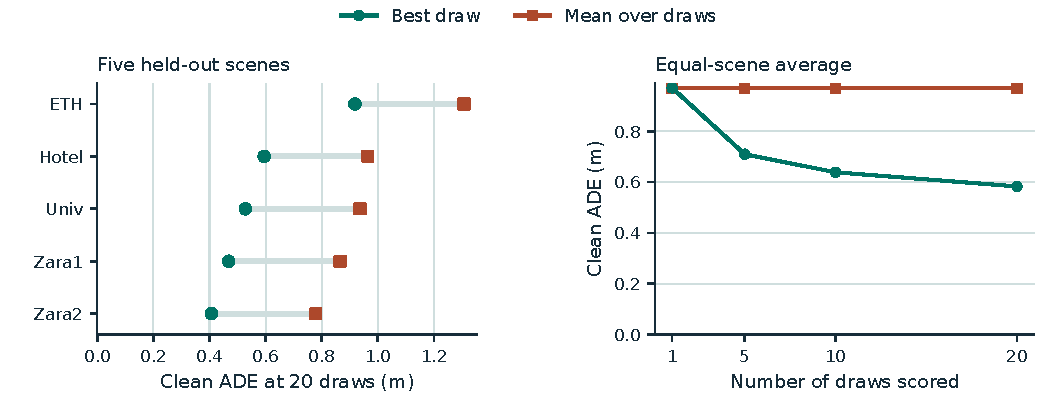
\includegraphics[width=.95\linewidth,height=.65\textheight,keepaspectratio]{contributions/social_stgcnn/assets/clean_sampling.pdf}
\par\smallskip
\begin{minipage}{.94\linewidth}
\small The same forecasts were scored at four sample budgets. With twenty
draws, meanADE was \textbf{0.940 m}. Five scenes carry equal weight.
\end{minipage}
\end{frame}

\begin{frame}{All twenty paths missed this reversal}
\centering
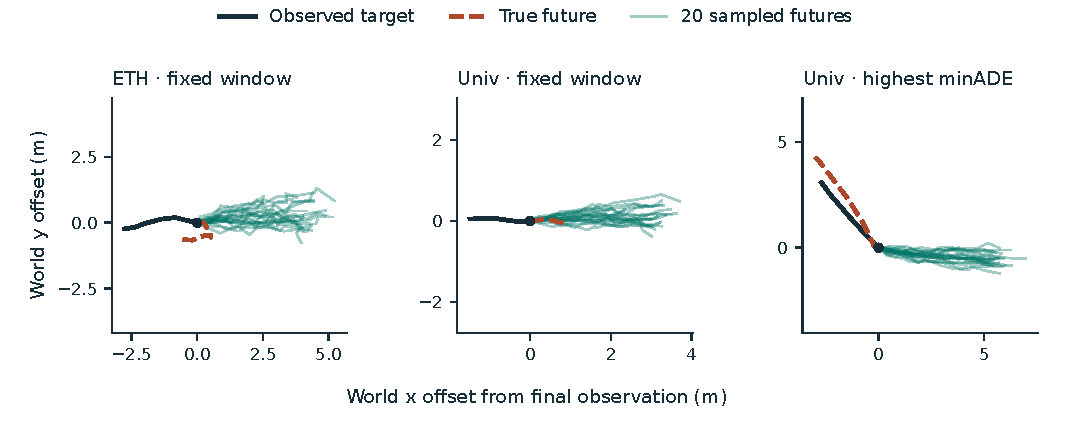
\includegraphics[width=.97\linewidth,height=.64\textheight,keepaspectratio]{contributions/social_stgcnn/assets/trajectories.pdf}
\par\smallskip
\begin{minipage}{.94\linewidth}
\small The right panel shows the largest clean minADE at seed zero. The target had
23 visible neighbors. Even the nearest forecast endpoint was
\textbf{9.52 m} from the observed destination.
\end{minipage}
\end{frame}
\endgroup
